section{Theoretische Grundlagen}

\subsection{Grundlagen der Festkörperphysik}
Für die Rastertunnelmikroskopie ist die räumliche Verteilung der Elektronen an 
der Oberfläche von zentraler Bedeutung. Die Blochtheorie macht Aussagen über 
die Aufenthaltswahrscheinlichkeiten von Elektronen in periodischen 
Gittern und liefert ein Modell zur Erklärung des Bändermodells. 
Für ein Elektron mit Wellenfunktion $\psi$ gilt bei Vernachlässigung der 
Elektron-Elektron-Wechselwirkung in der nichtrelativistischen Näherung die 
Schrödingergleichung 
\begin{equation}
    \Big[ - \frac{\hbar^2}{2m} \Delta + E_{\mathrm{pot}}(\mathbf{r}) \Big] \psi = E \psi
\end{equation}
mit periodischer potentieller Energie 
\begin{equation}
    E_{\mathrm{pot}}(\mathbf{r}) = E_{\mathrm{pot}}(\mathbf{r + R})
\end{equation}
in Richtung $\mathbf{R} = m \,\mathbf{a_1} + n \,\mathbf{a_2} + o \,\mathbf{a_3}, 
\quad m, n, o \in \mathbb{N}$, also den Vektoren zwischen den Gitterpunkten. 
Für die Lösung machen wir den Ansatz die sog. Blochwellenfunktionen
\begin{eqnarray}
    \psi(\mathbf{r}) = u(\mathbf{r}) \cdot \mathrm{e}^{-i \mathbf{k \cdot R}} \\
    \mathrm{mit} \quad u(\mathbf{r}) = u(\mathbf{r + R}) \nonumber
\end{eqnarray}
Für die Aufenthaltswahrscheinlichkeit folgt $|\psi(\mathbf{r})|^2 = |u|^2$. 

Wir gehen in unserer Beschreibung der untersuchten Metalle und Halbleiter 
vom Bändermodell aus. Durch die gegenseitige Beeinflussung der Atome im Gitter
werden die im Einzelatom noch stark voneinander abgetrennten Energie-Eigenzustände
der Elektronen aufgespalten und folgen so dicht aufeinander, dass Elektronen 
sehr leicht zwischen den einzelnen Zuständen wechseln können. Die atomaren
Energieniveaus bleiben jedoch zum Großteil soweit getrennt, dass klar definierte
"Bänder" entstehen. Das für $T = 0\deg K$ äußere Energieband ist das Valenzband.
Die zur chemischen Bindung beitragenden Elektronen gehören genau diesem Band an 
(Valenz = Bindung, Valenzelektronen). Das über dem Valenzband liegende Band wird 
als Leitungsband bezeichnet. Elektronen im Leitungsband sind räumlich nicht mehr 
gebunden, da sich die Orbitale der jeweiligen Atome überlagern – diese Elektronen 
können daher leicht Energie eines elektrischen Feldes aufnehmen und sich in dem 
Gitter bewegen. \\

\subsection{Charakterisierung von Kristallgittern}
Vor der Beschreibung der Oberflächen von Kristallen wenden wir uns dem darunter liegenden 
Gitter zu, das die Basis für die Oberfläche darstellt. Die charakteristischen Größen 
sind auch für die Oberflächen wichtig. Die Untersuchung der Kristallgitter findet vor 
Allem durch Beugungsexperimente statt, da diese die periodische Struktur am besten 
Ausnutzen und so zu höherer Genauigkeit kommen, als direkte Abbildung der Oberflächen. 
Für die gemessene Intensität $I(\mathbf{K})$ gilt für große Abstände $\mathbf{R}$ 
zwischen Strahlungsquelle und streuendem Medium sowie $\mathbf{R'}$ zwischen Streuer 
und Schirm am Ort B:
\begin{equation}
    I(\mathbf{K}) \propto |A_B|^2 \propto |\int \rho(\mathbf{r}) \mathrm{e}^{-i 
    \mathbf{K} \cdot \mathbf{r}} \mathrm{d}\mathbf{r}|^2
\end{equation}
Dabei ist $|A_B|$ die Amplitude der gemessenen Wellen am Schirm, $\rho (\mathbf{r})$ die 
komplexe Streudichte an Position $\mathbf{r}$ (siehe Abb.~\ref{fig:scatter_geometry}) 
und  $\mathbf{K} = \mathbf{k} - \mathbf{k_0}$ der Streuvektor, $\mathbf{k_0}$ der 
k-Vektor der auf das Streumedium auftreffenden Wellen und $\mathbf{k}$ der k-Vektor 
der am Schirm auftreffenden Welle. Für ein periodisches Gitter ist auch die Streudichte
periodisch und lässt sich daher in eine Fourierreihe zerlegen:
\begin{eqnarray}
    \rho(\mathbf{r}) = \sum_{\mathbf{G}} \rho_{\mathbf{G}} \mathrm{e}^{i \mathbf{G} 
        \cdot \mathbf{r}} \\
    \mathbf{r} = n_1 \mathbf{a_1} + n_2 \mathbf{a_2} + n_3 \mathbf{a_3} \\
    \mathbf{G} \cdot \mathbf{r}= 2 \pi m  \\
    n_1, \, n_2, \, n_3, \, m \in \mathbb{N}
\end{eqnarray}
Daraus folgt, dass der Vektor $\mathbf{G}$ als ganzzahlige Linearkombination 
reziproker Gittervektoren $\mathbf{g_i}$ mit der folgenden Bedingung darstellbar ist:
\begin{eqnarray}
    \mathbf{G} = h \mathbf{g_1} + k \mathbf{g_2} + l \mathbf{g_3} \\
    \mathbf{g_i} \cdot \mathbf{a_j} = 2 \pi \delta_{ij}
\end{eqnarray}
Schließlich lassen sich die Basisvektoren des reziproken Gitters berechnen:
\begin{equation}
    \mathbf{g_1} = 2 \pi \frac{\mathbf{a_2 \times a_3} }
        {\mathbf{a_1\cdot (a_2 \times a_3)}}
\end{equation}
Der Zusammenhang mit den experimentell messbaren Daten für $\mathbf{K}$ ist dann wie 
folgt gegeben:
\begin{equation} \label{eqn:G=K}
    I\,(\mathbf{K}) \propto \frac{|A_0|^2}{R'^2} \Big| \sum_{\mathbf{G}} \rho_{\mathbf{G}} 
    \int \mathrm{e}^{i \mathbf{(G - K) \cdot r}} \mathrm{d} \mathbf{r} \Big|^2
\end{equation}
Im Grenzwert unendlich ausgedehnten Volumens wird das Integral zur Deltafunktion, sodass 
für die Intensität gilt:
\begin{equation}
    I\,(\mathbf{K = G}) \propto \frac{|A_0|^2}{R'^2} \,|\rho_{\mathbf{G}} |^2 \, V
\end{equation}

Bei der Bezeichnung von Oberflächen werden die sogenannten Millerschen Indizes benutzt. 
Spannt man mit drei nicht auf einer Geraden liegenden Gitterpunkten, so ist diese durch 
drei ganze Zahlen $m, n, o$ gekennzeichnet. Aus diesen erhält man ein teilerfremdes 
Triplet $(h, k, l)$, indem man die reziproken Werte $h' = 1/m, k' = 1/n, l' = 1/o$ mit 
einer ganzen Zahl $p$ multipliziert. Es lässt sich nun zeigen, dass der reziproke 
Gittervektor $\mathbf{G}$ senkrecht auf dem mit $(h, k, l)$ beschriebenen Gitter steht, 
und für die die in \ref{eqn:G=K} gegebene Bedingung $\mathbf{G = K}$ die Braggsche Reflexionsbedingung 
\begin{equation}
    \gamma = 2 d_{hlk} \sin \Theta
\end{equation}
gilt, wobei 
\begin{equation}
    d_{hkl}=2 \pi / |G_{hkl}|
\end{equation}
der Netzebenenabstand ist und der $\Theta$ der in Abb.~\ref{fig:Bragg_Winkel} definierte
Glanz- oder Braggwinkel ist



\begin{figure}
    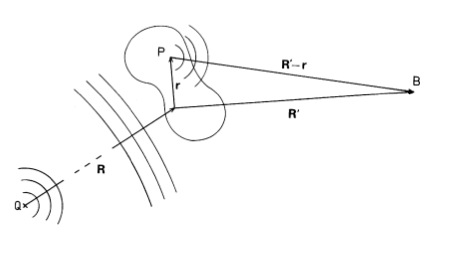
\includegraphics[width=1.0\textwidth]{pics/scatter_geometry}
    \caption{Zur Herleitung der Streukinematik
aus \cite{ibach2009festkorperphysik} }
    \label{fig:scatter_geometry}
\end{figure}

\begin{figure}
    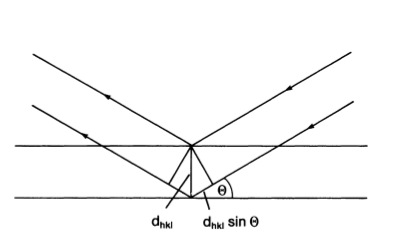
\includegraphics[width=1.0\textwidth]{pics/Bragg_Winkel}
    \caption{Zur Definition des Braggwinkels $\Theta$. Die Netzebenen haben einem Abstand 
von $d_{hlk}$.  
aus \cite{ibach2009festkorperphysik} }
    \label{fig:Bragg_Winkel}
\end{figure}


\subsection{Grundlagen der Festkörperoberflächen}
Das zuvor angenommen, unendlich ausgedehnte, periodische Kristallgitter spielt 
bei der Untersuchung der Oberflächen nur noch eine untergeordnete Rolle – 
schließlich ist eine Oberfläche zunächst einmal eine Abweichung dieser 
Eigenschaft. Im Allgemeinen kann es Abweichungen in null, ein, zwei oder drei 
Dimensionen geben. Letztere sind Abweichungen der unterliegenden Baustruktur, 
die zum Teil eine Mosaikstruktur bilden, die sich auch auf größere Skalen 
erstrecken. Zweidimensionale Strukturen tauchen als großflächige 
Überstrukturen oder kleinere Facetten auf. Eine Kategorisierung verschiedener 
Oberflächen wird von Henzler und Göpel \cite{henzler1991oberflachenphysik} 
gegeben (Abb.:~\ref{fig:oberflaeche}).
In jedem Fall erfahren die Atome der Oberfläche erfahren nicht mehr das 
regelmäßige Potential von allen Seiten. Die resultierenden Veränderung werden je 
nach Art als Oberflächenrelaxation oder -rekonstruktion. 
Ersteres bezeichnet lediglich eine globale Verschiebung der oberen Schicht 
gegen die Basis, beispielsweise normal oder lateral, wobei die Symmetrien 
der Oberfläche nicht verändert werden und sich die freie Energie verringert. 
Dieser Effekt wird bei den meisten Metallen beobachtet \cite{oura2003surface}. 
Abb. \ref{fig:Ag(110)} zeigt beispielsweise die relaxierte Oberfläche von Silber 
auf der (110)-Fläche.
Bei der Oberflächenrekonstruktion bilden sich meist größere Einheitszellen, als die 
des darunter liegenden Kristalls. Bei Halbleitern hängt das oft damit zusammen, 
dass die Anzahl nicht abgesättigter Bindungen minimiert wird, so beispielsweise 
bei Silizium entlang der (100)-Fläche, bei der nach gedanklichem Aufspalten zwei 
Bindungen frei wären. Je zwei Atome verbinden sich zu sog. Dimeren, wobei die 
Oberfläche räumlich verzogen wird und sich volle bzw. leere Reihen mit einer 
Höhe von bis zu fünf Schichten und über große Entfernungen bilden 
\cite{chadi1979atomic}. Die bereits in der historischen Einleitung gezeigte 
Si-Oberfläche entlang der 
(111)-Ebene zeigt ebensfalls eine Oberflächenrekonstruktion, allerdings mit 
deutlich anderen Mustern. Die kubisch-flächenzentrierten Edelmetalle der 
6.~Periode, Ir, Pt und Au bilden als Ausnahme unter den Metallen ebenfalls 
Oberflächenrekonstruktionen, die sog. \emph{missing row}-Konstruktion, 
wie weiter unten bei der Beschreibung von Gold verdeutlicht wird 
\cite{kittel2013einfuhrung}. 

\begin{figure}
    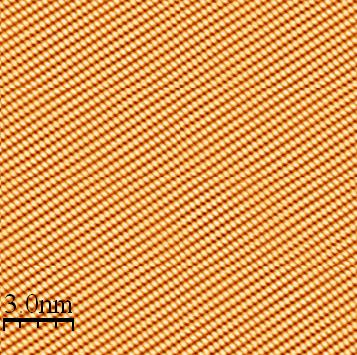
\includegraphics[width=1.0\textwidth]{pics/Ag(110)_clean}
    \caption{Rastertunnelkikroskop-Aufnahme mit atomare Auflösung einer reinen 
Silberoberfläche entlang der (110)-Fläche. Zu erkennen ist, dass die Oberfläche 
lediglich relaxiert ist, und Rekonstruktion stattfindet. 
Aus \cite{kahn:stm_images}.}
    \label{fig:Ag(100)}
\end{figure} 

Zur mathematischen Beschreibung regelmäßiger Überflächen werden die Gittervektoren 
aus dem Ortsraum benutzt, die in der Oberfläche liegen. Ausreichend sind meistens 
jene aus der obersten Atomschicht. Die Atome befinden sich dann an den Positionen 
\begin{equation}
    \mathbf{r} = m_1 \mathbf{a_1} + m_2 \mathbf{a_2},
\end{equation}
wobei nach Konvention $|\mathbf{a_1}| \le |\mathbf{a_2}|$ und 
$\gamma = \angle (\mathbf{a_1}, \mathbf{a_2}) > 90 \deg$ der Winkel zwischen den 
beiden Vektoren ist. Da die Atom in einer Ebene liegen, ist die Anzahl möglicher 
Anordnungen, die sog. Bravais-Netze, deutlich kleiner als für einen 3D-Kristall. 
Es gibt genau fünf, wie in Abb.~\ref{fig:Bravais} gezeigt 
\cite{henzler1991oberflachenphysik}.
Zur vollständigen Beschreibung fehlen dann allerdings noch die Angaben zur Lage 
der Oberflächenatome relativ zur darunter befindlichen Basis. 

Zur Beschreibung der Oberfläche wird zuerst die ideale Oberfläche angenommen, 
die sich aus dem darunter liegenden Kristallgitter ergäbe, und deren Vektoren mit
$|\mathbf{a_1}| \le |\mathbf{a_2}|$ bezeichnet werden. Die tatsächle Struktur, 
soweit periodisch, kann dann als Verhältnisse $\frac{\mathbf{a_1}}{\mathbf{b_1}}$, 
$\frac{\mathbf{a_1}}{\mathbf{b_1}}$ und Winkel zwischen Basis und Oberfläche angegeben 
werden. Zusammen mit der Millerschen Schreibweise für die Kristallfläche der Basis 
ergibt sich so eine kompakte Schreibweise, z.~B. 
$\mathrm{Si}(111)(\sqrt{3} \times \sqrt{3}) \mathrm{R} 30 \deg$. 
Ist diese Schreibweise ungeeignet aufgrund fehlender Symmetrien, so kann eine 
Matrixschreibweise benutzt werden. Sind die Einträge ganze Zahlen, so liegen die 
Atome der Oberfläche direkt auf der Basis. Bei rationalen Zahlen gibt es auch 
zwischen den Basisatomen Oberflächenatome, während bei irrationalen Zahlen die 
Oberfläche quasi unabhänging von der Basis gesehen werden muss. Sie wird dann auch 
als inkommensurabel bezeichnet. \cite{henzler1991oberflachenphysik}

\begin{figure}
    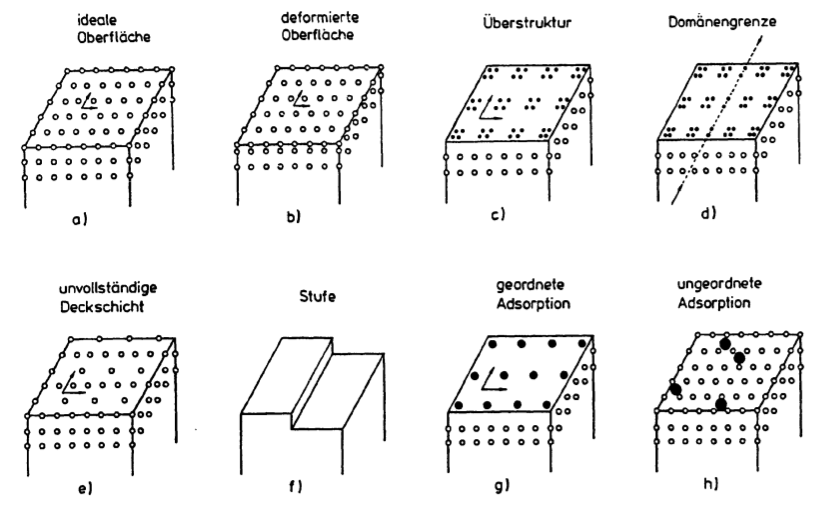
\includegraphics[width=1.0\textwidth]{pics/oberflaechenstruktur}
    \caption{Die ideale Oberfläche und einige mögliche Oberflächenstrukturen. 
Die ideale Oberfläche entspricht einer Gitterebene im Kristall, die defomierte 
Oberfläche entsteht durch Relaxation (hier in normaler Richtung) und wird bei den 
meisten Metallen beobachtet, während die Überstruktur ein Resultat der Rekonstruktion 
ist und z. B. bei Halbleitern oder Gold zu beobachten ist. 
Aus \cite{henzler1991oberflachenphysik} }
    \label{fig:oberflaeche}
\end{figure} 
\begin{figure}
    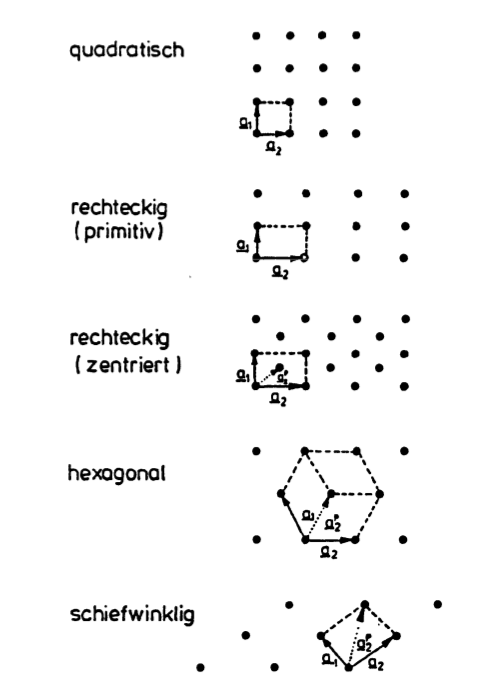
\includegraphics[width=0.5\textwidth]{pics/Bravais}
    \caption{Bravais-Gitter zur Oberflächenstrukturbeschreibung. Die kleinstmöglichen
Zellen sind in den unteren drei Gittern mit $\underline{a}_2^p$ beschriftet. 
Aus \cite{henzler1991oberflachenphysik} }
    \label{fig:Bravais}
\end{figure} 


\subsection{Struktur von Graphit, Gold und $\mathrm{MoS_2}$}
Die Kristallstruktur von Graphit zeichnet sich vor allem durch seine Schichtenstruktur 
aus. Die Kohlenstoffatome sind in den aus kovalent gebundenen Sechsecken bestehenden 
Basalebenen oder Graphenschichten deutlich fester aneinander gebunden (4.3 eV), als 
an solche aus benachbarten Schichten (0.07 eV). Daher ist Graphit entlang dieser Linien 
sowohl mechnisch deutlich stabiler als auch sehr viel leitfähiger (für Wärme und 
elektrischen Strom). Die Unterschiede in der Bindungsenergie spiegeln sich auch in den 
Abständen wider: So sind nächsten Nachbarn innerhalb einer Schicht nur $0.142\mathrm{nm}$ 
entfernt, während die Schichten $0.335\mathrm{nm}$ auseinander liegen.  
Graphit tritt nicht nur in zueinander korrlierten Schichten auf, 
sondern auch unkorrliert (sog. turbostratischer Kohlenstoff). Die hier untersuchte Form 
ist jedoch regelmäßig - die Winkelabweichung für das verwendete HOPG (highly orientated 
pyrolytic graphite) beträgt weniger als $1 \deg$ \cite{mcnaught2000iupac}. Diese 
synthetische Form des Graphit wird auf Grund von ihrer Regelmäßigkeit und Reinheit 
heute zur Kalibrierung von Rastertunnelmirkoskopen verwendet \cite{lapshin1998automatic}. 
Es liegen in der Schichtung jedoch nicht alle Atome übereinander, sondern lediglich 
jedes zweite aus jedem Sechseck (siehe Abb.~\ref{fig:graphite}). 
Dadurch kommt es an der Oberfläche zu einem oft beobachteten 
Effekt: Anstatt sämtliche Atome der Sechsecke zu beobachten, taucht nur die Hälfte auf 
den STM-Bildern auf. Erklärt wird das dadurch, dass die Elektronendichte in der 
Fermienergie für Atome mit Nachbarn darunter höher liegt als bei solchen ohne
\cite{zeinalipour2008new}. Selloni~et~al.~\cite{Sellino1985} berechneten den Abstand 
der Atome mit bzw. ohne direkten Nachbarn in der Schicht darunter mit $0.15 \AA$. 

\begin{figure}
    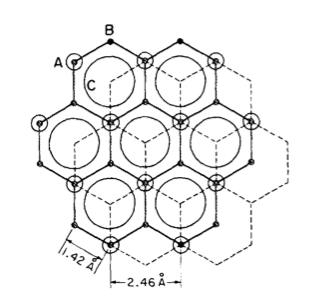
\includegraphics[width=1.0\textwidth]{pics/graphite}
    \caption{Hexagonale Oberflächenstruktur von Graphit. An den umkreisten Orten (A) 
liegen jeweils Atome aus der ersten und der zweiten Schicht übereinander, bei den 
übrigen (B) nicht. Bei STM-Aufnahmen sind fast ausschließlich die Atome mit Nachbarn 
zu erkennen, da hier Elektronen nahe der Fermienergie räumlich weiter oben liegen. 
Aus \cite{park1986tunneling}}
    \label{fig:graphite}
\end{figure} 

Gold ist als kubisch-flächenzentriertes Kristallgitter aufgebaut. Die Gitterkonstante 
beträgt $407.82\mathrm{pm}$\cite{ohring1995engineering}. Im Gegensatz zum Graphit 
treten jedoch beim Gold enorme Veränderungen der Oberflächenstruktur gegenüber der 
darunter liegenden Basis auf. Auf einer (110)-Fläche wurde die Bildung von 
(111)-Facetten beobachtetet, die Kanälevon meistens zwei bis vier Schichten Tiefe 
formen. Gleichzeitig ist die Oberfläche von Stufen gekennzeichnet, die sowohl parallel 
als auch normal zu den Kanälen verlaufen, siehe Abb. \ref{fig:Au(110)}. Die Darstellung 
der Oberfläche mit dem Rastertunnelmikroskop ist auf Grund der metallischen Struktur 
deutlich schwieriger als bei Halbleitern, da die Elektronen aus dem Leitungsband kaum 
räumlich lokalisiert sind. 

\begin{figure}
    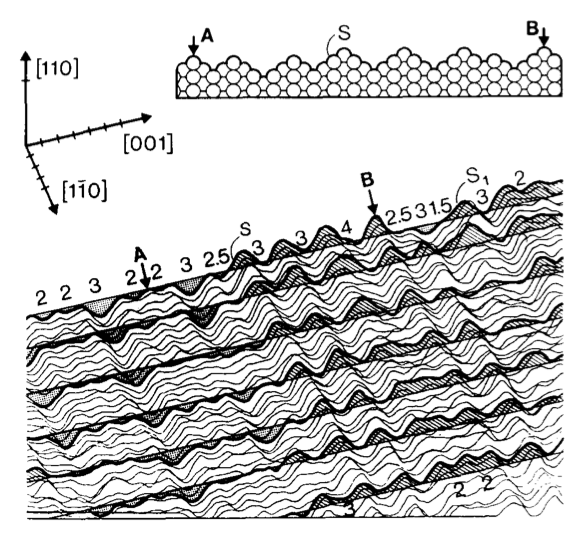
\includegraphics[width=1.0\textwidth]{pics/Au(110)_channels}
    \caption{Rastertunnelmikroskop-Aufnahmen von Gold(110)-Oberfläche mit 
Rekonstruktion. Die Geraden verdeutlichen die abschüssige Terassenstruktur, die 
Nummern die Tiefe der Kanäle (in Vielfachen der Ebenenabstände). Bei $\mathrm{S}$
und $\mathrm{S_1}$ befinden sich Stufen mit Höhe einer Atomlage. An den Kristallaxen 
ist der Maßstab gekennzeichnet: ein Schritt entsprechen 5 \AA. Über der Aufnahme 
deutet ein schematischer Querschnitt die Struktur der Kanäle an. 
Aus \cite{binnig1983111}.}
    \label{fig:Ag(100)}
\end{figure} 

Molybdänit ($\mathrm{MoS_2}$, auch Molybdän(IV)-sulfid) ist ein Halbleiter mit 
hexagonalem Kristallgitter der Raumgruppe $\mathrm{P \, 6_3/mmc}$. Ähnlich 
dem Graphit gibt es eine schichtartige Struktur, auch hier können die Schichten 
relativ leicht gegeneinander verschoben werden. Die Gitterparameter sind mit 
$a = 3.161 \AA$ sowie $c = 12.295 \AA$ angegeben, siehe
Abb.~\ref{fig:MoS2_structure} \cite{schrocke1981mineralogie}. 
Auf Gund der Schichtstruktur findet $\mathrm{MoS_2}$ als 
Schmiermittel Verwendung und kann wie Graphen als einatomige Schicht isoliert 
werden, sodass es mögliches Transitormaterial gehandelt wird 
\cite{mak2010atomically}. 

\begin{figure}
    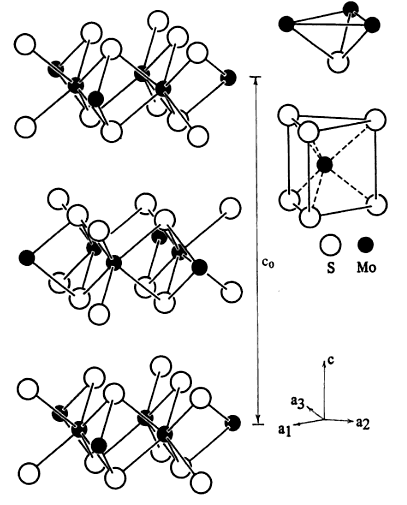
\includegraphics[width=1.0\textwidth]{pics/MoS2_structure}
    \caption{Gitterstruktur von $\mathrm{MoS_2}$, Ausschnitte aus drei übereinander 
liegenden Schichten mitsamt Koordinationspolyedern. Für die Abstände gilt 
$a_1 = a_2 = a_3 = 3.161\AA =: a$ und $c_0 = 12.295\AA$. 
Aus \cite{schrocke1981mineralogie}.}
    \label{fig:MoS2_structure}
\end{figure} 
